
% \part*{Appendices}
% \counterwithin{figure}{section}
% \counterwithin{table}{section}
% \counterwithin{equation}{section}


% \section{Additional Pointers for Future Work}

% In addition to future work discussed in Section~\ref{sec:discussion}, here we list other promising directions for future work. 
% Given the strong performance of transformers, we suspect that offline Q-learning with a transformer architecture is a promising future direction. Furthermore, there are several avenues for future investigation related to the ablation studies in Section~\ref{sec:ablation} for key design choices in scaled Q-learning: (1) it is unclear if C51 works better because of the distributional formulation or the categorical representation and experiments with other distributional formulations could answer this question, (2) we did not extensively try alternate feature normalization schemes, which may improve results. Another important avenue for future work is to scale offline Q-learning on other RL domains such as robotic navigation, manipulation, locomotion, education, etc.
% This would require building large-scale tasks, and we believe that scaled QL would provide for a good starting point for scaling in these domains. Finally, in line with \citet{agarwal2022beyond}, we plan to release our pre-trained models, which we hope would enable subsequent methods to build upon.

\section{Additional Results for Scaled Q-Learning}


\begin{figure}[H]
    \centering
    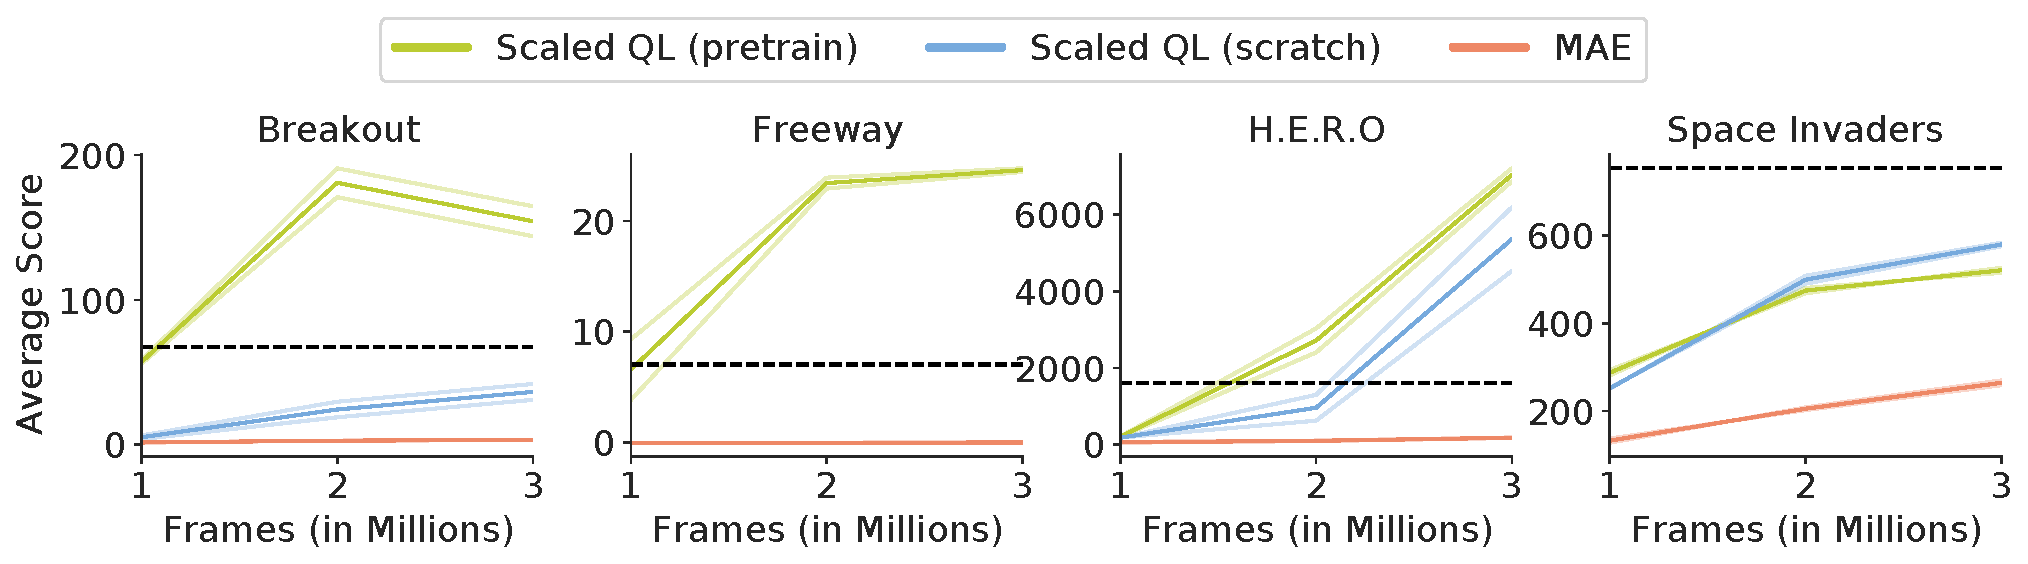
\includegraphics[width=\linewidth]{chapters/scaled_ql/figures/online_ft_curve.pdf}
    \vspace{-0.4cm}
    \caption{Learning curves for \textbf{online fine-tuning on unseen game variants}. The dotted horizontal line shows the performance of a single-game DQN agent trained for 50M frames (16x more data than our methods). See Figure~\ref{fig:online_ft} for visualization of the variants.}
    \label{fig:lr_curves_online_ft}
\end{figure}


\begin{figure}[h]
    \vspace{-0.5cm}
    \centering
    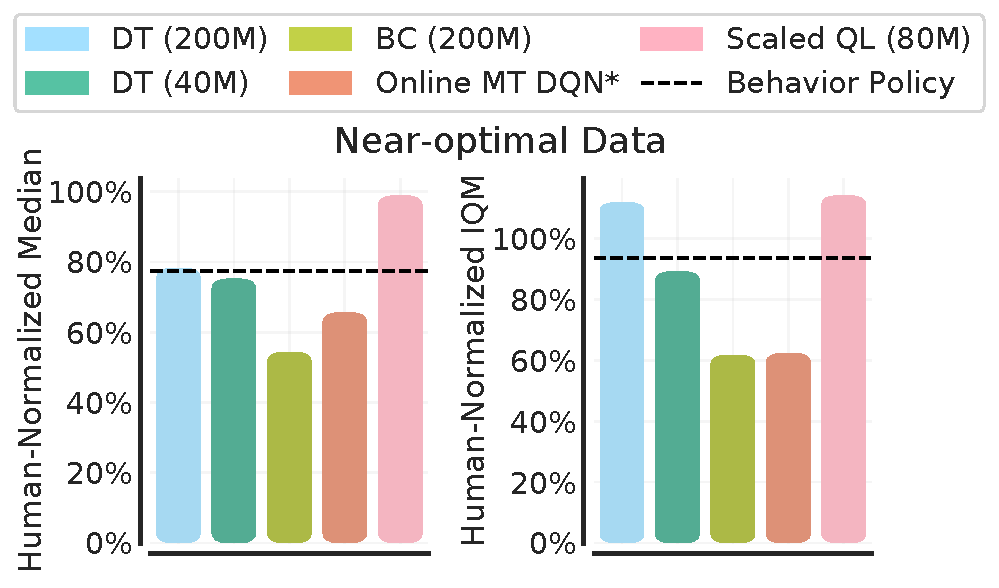
\includegraphics[width=0.6\linewidth]{chapters/scaled_ql/figures/full_data_results.pdf}
    \vspace{-0.25cm}
    \caption{\footnotesize{\textbf{Offline scaled conservative Q-learning vs other prior methods} with near-optimal data. Scaled QL outperforms the best DT model, attaining an IQM human-normalized score of \textbf{114.1\%} and a median human-normalized score of \textbf{98.9\%} compared to 111.8\% and 78.2\% for DT, respectively.}}
    \label{fig:full_data_results}
    \vspace{-0.2cm}
\end{figure}

\subsection{{{Results for Scaling Discrete-BCQ}}} 
\label{app:discrete_bcq}
{To implement discrete BCQ, we followed the official implementation from \citet{fujimoto2019benchmarking}. We first trained a model of the behavior policy, $\widehat{\pi}_\beta(\mathbf{a}|\bs)$, using an architecture identical to that of the Q-function, using negative log-likelihood. Then, following \citet{fujimoto2019benchmarking}, we updated the Bellman backup to only perform the maximization over actions that attain a high likelihood under the probabilities learned by the behavior policy, as shown below:}
\begin{align*}
    {y(\bs, \mathbf{a}) := r(\bs, \mathbf{a}) + \gamma \max_{\mathbf{a}': \widehat{\pi}_\beta(\mathbf{a}'|\bs') \geq \tau \cdot \max_{\mathbf{a}''} \widehat{\pi}_\beta(\mathbf{a}''|\bs')} {Q}(\bs', \mathbf{a}')},
\end{align*}
{where $\tau$ is a hyperparameter. To tune the value of $\tau$, we ran a preliminary initial sweep over $\tau=\{0.05, 0.1, 0.3\}$. When using C51 in our setup, we had to use a smaller CQL $\alpha$ of 0.05 (instead of 0.1 for the MSE setting from \citet{kumar2021dr3}), possibly because a discrete representation of Q-values used by C51 is less prone to overestimation. Therefore, in the case of discrete-BCQ, we chose to perform an initial sweep over $\tau$ values that were smaller than or equal to (i.e., less conservative) the value of $\tau=0.3$ used in \citet{fujimoto2019benchmarking}.} 

{Since BCQ requires an additional policy network, it imposes a substantial memory overhead and as such, we performed a sweep for initial 20 iterations to pick the best $\tau$.
We found that in these initial experiments, $\tau=0.05$ performed significantly worse, but $\tau=0.1$ and $\tau=0.3$ performed similarly. So, we utilized $\tau=0.3$ for reporting these results.}

\begin{figure}
    \centering
    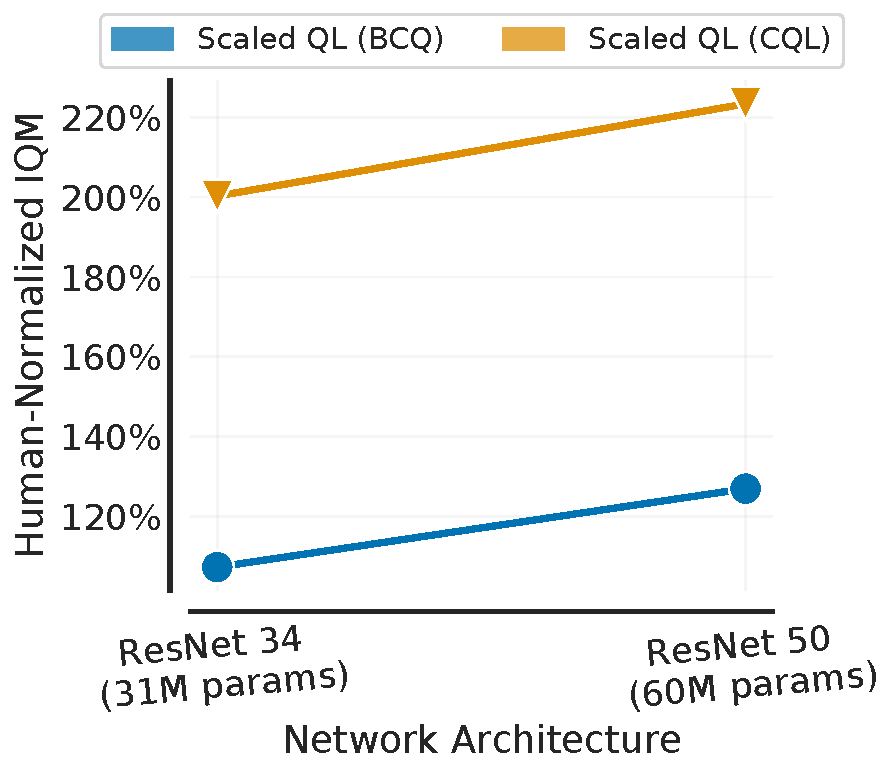
\includegraphics[width=0.5\linewidth]{chapters/scaled_ql/appendix_figures/bcq_vs_cql.pdf}
    \caption{\footnotesize{{\textbf{Performance of scaling CQL and BCQ in terms of IQM human-normalized score.} We perform this comparison on the six-game setting for 100 epochs (note that these results are after 2x longer training than other ablations in Table~\ref{tab:ablation_dr3}). Observe that for discrete-BCQ the performance improves from ResNet 34 to ResNet 50, indicating that it does scale favorably as network capacity increases.}}}
    \label{tab:ablation_bcq}
    \vspace{-0.1cm}
\end{figure}


{We ran these scaling experiments with ResNet 34 and ResNet 50 in the six-game setting and report human-normalized IQM performance after 100 epochs = 6.25M gradient steps in Figure~\ref{tab:ablation_bcq}. We also present the results for CQL on the side for comparisons. Observe that we find favorable scaling trends for BCQ: average performance over all games increases as the network size increases, indicating that other offline RL algorithms such as BCQ can scale as we increase network capacity.} 

\vspace{-0.2cm}
\subsection{{{Ablation for Backbone Architecture}}}
\label{app:backbone_ablation}
\vspace{-0.2cm}
{In this section, we present some results ablating the choice of the backbone architecture. For this ablation, we ablate the choice of the spatial embedding while keeping group normalization fixed in both cases. We perform this study for the 40-game setting. Observe that using the learned spatial embedding results in better performance, and improves in 27 out of 40 games compared to not using the learned embeddings.}

\begin{table}[h]
    \centering
% \fontsize{8}{8}\selectfont
    \centering
    \vspace{-0.4cm}
    \caption{\footnotesize{{\textbf{Ablations for the backbone architecture in the 40-game setting} with ResNet 101. Observe that learned spatial embeddings leads to around 80\% improvement in performance.}}} % (as large as 39.4\% improvement on human-median normalized score with ResNet 101).}}
    \label{tab:ablation_backbone_40_game}
    \vspace{0.25cm}
\resizebox{0.99\textwidth}{!}{\begin{tabular}{l@{}cc@{}}
\toprule
 & \textbf{Scaled QL without backbone} & \textbf{Scaled QL w/ backbone} \\
\midrule
\textbf{Median human-normalized score} & 54.9\% & \textbf{98.9}\% \\
\textbf{IQM human-normalized score}  &  68.9\% & \textbf{114.1}\% \\
\midrule
\textbf{Num. games with better performance} & 13 / 40 & \textbf{27 / 40} \\
\bottomrule
% \vspace{-0.15in}
\end{tabular}}
\end{table}

{Regarding the choice of group normalization vs batch normalization, note that we have been operating in a setting where the size of the batch per device / core is only 4. Particularly, we use Cloud TPU v3 accelerators with 64 / 128 cores, and bigger batch sizes than 4 do not fit in memory, especially for larger-capacity ResNets. This means that if we utilized batch normalization, we would be computing batch statistics over only 4 elements, which is known to be unstable even for standard computer vision tasks, for example, see Figure 1 in \citet{wu2018group}.} 

\vspace{-0.2cm}
\subsection{{{Results for Scaled QL Without Pessimism}}}
\label{app:no_pessimism}
\vspace{-0.2cm}
{In Table~\ref{tab:ablation_no_pessimism}, we present the results of running scaled Q-learning with no conservatism, i.e., by setting the value of $\alpha$ in CQL training to 0.0 in the six game setting. We utilize the entire DQN-replay dataset~\citep{agarwal2019optimistic} for each of these six games that would be present in the full 40-game dataset, to preserve the per-game dataset diversity.}

{Observe that while utilizing no conservatism does still learn, the performance of scaled QL without conservatism is notably worse than standard scaled QL. Interestingly, on \textsc{Asterix}, the performance without pessimism is better than performance with pessimism, whereas, the use of pessimism in \textsc{SpaceInvaders} and \textsc{Seaquest} leads to at least 2x improvement in performance.}

\begin{table}[h]
    \centering
% \fontsize{8}{8}\selectfont
    \centering
    \vspace{-0.1cm}
    \caption{\footnotesize{{\textbf{Performance of scaled QL with and without conservatism in terms of IQM human-normalized score} in the six-game setting for 100 epochs (2x longer training compared to other ablations in Table~\ref{tab:ablation_dr3}) performed with a ResNet 50. Observe that utilizing conservatism via CQL is beneficial. We also present per-game raw scores in this table. Observe that while in one games no pessimism with such data can outperform CQL, we do find that overall, conservatism performs better.}}} 
    \label{tab:ablation_no_pessimism}
    \vspace{0.35cm}
\resizebox{0.85\textwidth}{!}{\begin{tabular}{l@{}cc@{}}
\toprule
 & \textbf{Scaled QL without CQL} & \textbf{Scaled QL w/ CQL} \\
\midrule
\textsc{Asterix} & 38000 &	35200 \\
\textsc{Breakout} & 322	& 410 \\
\textsc{Pong} & 12.6 & 19.8 \\
\textsc{Qbert} & 13800	& 15500 \\
\textsc{Seaquest} & 1378 &	3694 \\
\textsc{SpaceInvaders} & 1675 & 3819 \\
\midrule
\textbf{IQM human-normalized score}  & 188.3\% & \textbf{223.4\%} \\
\bottomrule
% \vspace{-0.15in}
\end{tabular}}
\end{table}

{We also present some results without pessimism in the complete 40-game setting in Table~\ref{tab:ablation_no_pessimism_40_game}. Unlike the smaller six game setting, we find a much larger difference between no pessimism (without CQL) and utilizing pessimism via CQL. In particular, we find that in 6 games, not using pessimism leads to slightly better performance, but this strategy hurts in all other games, giving rise to an agent that performs worse than random in many of these 34 games. This indicates that pessimism is especially deisrable as the diversity of tasks increases.}

\begin{table}[h]
    \centering
% \fontsize{8}{8}\selectfont
    \centering
    \vspace{-0.1cm}
    \caption{\footnotesize{{\textbf{Scaled QL with and without conservatism in terms of IQM human-normalized score in the 40-game setting} with ResNet 101. Observe that utilizing conservatism via CQL is still beneficial.}}} 
    \label{tab:ablation_no_pessimism_40_game}
    \vspace{0.25cm}
\resizebox{0.85\linewidth}{!}{\begin{tabular}{lcc}
\toprule
 & \textbf{Scaled QL without CQL} & \textbf{Scaled QL w/ CQL} \\
\midrule
\textbf{Median human-normalized score} & 11.1\% & 98.9\% \\
\textbf{IQM human-normalized score}  &  13.5\% & 114.1\% \\
\midrule
\textbf{Num. games with better performance} & 6 / 40 & \textbf{34 / 40} \\
\bottomrule
% \vspace{-0.2in}
\end{tabular}}
\end{table}

\vspace{-0.2cm}
\section{Implementation Details and Hyper-Parameters}
\vspace{-0.2cm}

In this section, we will describe some of the implementation details behind our method and will provide implementation details for our approach, including the details of the network architectures, the details of feature normalization and the details of our training and evaluation protocol.

\subsection{Network Architecture}
\label{sec:arch}

In our primary experiments, we consider variants of ResNet architectures for scaled Q-Learning. The vision backbone in these architectures mimic the corresponding ResNet architectures from \citet{resnet}, however, we utilize group normalization~\citep{wu2018group} (with a group size of 4) instead of batch normalization, and instead of applying global mean pooling to aggregate the outputs of the ResNet, we utilize learned spatial embeddings~\citep{kumar2022pre}, that learn a matrix that point-wise multiplies the output feature map of the ResNet. The output volume is then flattened to be passed as input to the feed-forward part of the network. The feed-forward layer part of the network begins with a layer of size 2048, and then applies layer norm on the network. After this we apply 3 feed-forward layers with hidden dimension 1024 and ReLU activations, to obtain the image representation 

Then, we apply feature normalization to the representation, by applying a normalization layer which divides the representation of a given observation by its $\ell_2$ norm. Note that we do pass gradients through this normalization term. Now, this representation is passed into different heads that are supposed to predict the Q-values. 
The total number of heads is equal to the number of games we train on. Each head consists of a linear layer that maps the 1024-dimensional normalized representation to a vector of $K$ elements, where $K = |\mathcal{A}|$ (i.e., the size of the action space) for the standard real-valued parameterization of Q-values, and $K = |\mathcal{A}| \times 51$ for C51. The network does not apply any output activation in either case, and the Q-values are treated as logits for C51.  

\subsection{Details of C51}
\label{sec:c51_details}

For the main results in the chapter, we utilize C51. The main hyperparameter in C51 is the size of the support set of Q-values. Unlike the paper from \citet{bellemare2017distributional} which utilizes a support set of $[-10, 10]$, we utilize a support set of $[-20, 20]$ to allow for flexibility of CQL: Applying the CQL regularizer can underestimate or overestimate Q-values, and this additional flexibility aids such scenarios. Though, we still utilize only 51 atoms in our support set, and the average dataset Q-value in our training runs is generally always smaller, around $\sim 8-9$.

\subsection{Training and Evaluation Protocols and Hyperparameters}

We utilize the initial 20\% (sub-optimal) and 100\% (near-optimal) datasets from \citet{agarwal2019optimistic} for our experiments. These datasets are generated from runs of standard online DQN on stochastic dynamics Atari environments that utilize sticky actions, \ie\ there is a 25\% chance at every time step that the environment will execute the agents previous action again, instead of the new action commanded. The majority of the training details are identical to a typical run of offline RL on single-game Atari. We discuss the key differences below. 


We trained our ResNet 101 network for $10M$ gradient steps with a batch size of 512. The agent hasn't converged yet, and the performance is still improving gradually. When training on multiple games, we utilize a stratified batch sampling scheme with a total batch size of $512$. To obtain the batch at any given training iteration, we first sample 128 game indices from the set all games (40 games in our experiments) with replacement, and then sample $4$ transitions from each game. This scheme does not necessarily produce an equal number of transitions from each game in a training batch, but it does make sure that all games are seen in expectation throughout training.

Since we utilize a larger batch size, that is 16 times larger than the standard batch size of 32 on Atari, we scale up the learning rate from $5e-05$ to $0.0002$, but keep the target network update period fixed to the same value of 1 target update per $2000$ gradient steps as with single-task Atari. We also utilize $n$-step returns with $n=3$ by default, with both our MSE and C51 runs.

\begin{table*}[t]
\small
\caption{\textbf{Hyperparameters used by multi-game training.} Here we report the key hyperparameters used by the multi-game training. The differences from standard single-game training are highlighted in red.} 
\vspace{0.05cm}
\centering
\resizebox{0.8\textwidth}{!}{\begin{tabular}{lrr}
\toprule
Hyperparameter & \multicolumn{2}{r}{Setting (for both variations)} \\
\midrule
Eval Sticky actions && \textcolor{red}{No}        \\
Grey-scaling && True \\
Observation down-sampling && (84, 84) \\
Frames stacked && 4 \\
Frame skip~(Action repetitions) && 4 \\
Reward clipping && [-1, 1] \\
Terminal condition && Game Over \\
Max frames per episode && 108K \\
Discount factor && 0.99 \\
Mini-batch size && \textcolor{red}{512} \\
Target network update period & \multicolumn{2}{r}{every 2000 updates} \\
Training environment steps per iteration && 62.5k \\
Update period every && 1 environment steps \\
Evaluation $\epsilon$ && 0.001 \\
Evaluation steps per iteration && 125K \\
Learning rate && \textcolor{red}{0.0002} \\
n-step returns ($n$) && 3 \\
CQL regularizer weight $\alpha$ && 0.1 for MSE, 0.05 for C51\\
\bottomrule
\end{tabular}}
\label{table:hyperparams_atari}
\end{table*}

\textbf{Evaluation Protocol.} Even though we train on Atari datasets with sticky actions, we evaluate on Atari environments that do not enable sticky actions following the protocol from \citet{lee2022multi}. This allows us to be comparable to this prior work in all of our comparisons, without needing to re-train their model, which would have been too computationally expensive. Following standard protocols on Atari, we evaluate a noised version of the policy with an epsilon-greedy scheme, with $\varepsilon_\text{eval} = 0.001$. Following the protocol in \citet{castro2018dopamine}, we compute average return over 125K training steps. 

\subsection{Fine-Tuning Protocol}
\label{sec:finetuning}

\textbf{For offline fine-tuning} we fine-tuned the parameters of the pre-trained policy on the new domain using a batch size of 32, and identical hyperparameters as those used during pre-training. We utilized $\alpha=0.05$ for fine-tuning, but with the default learning rate of $5e-05$ (since the batch size was the default 32). We attempted to use other CQL $\alpha$ values $\{0.07, 0.02, 0.1\}$ for fine-tuning but found that retaining the value of $\alpha = 0.05$ for pre-training worked the best. For reporting results, we reported the performance of the algorithm at the end of 300k gradient steps.  

\textbf{For online fine-tuning}, we use the C51 algorithm~\citep{bellemare2017distributional}, with $n$-step$=3$ and all other hyperparameters from the C51 implementation in the Dopamine library ~\citep{castro2018dopamine}. We swept over two learning rates, $\{1e-05, 5e-05\}$ for all the methods and picked the best learning rate per-game for all the methods. For the MAE implementation, we used the Scenic library~\citep{dehghani2021scenic} with the typical configuration used for ImageNet pretraining, except using $84\times84\times4$ sized Atari observations, instead of images of size $224 \times 224 \times 3$. We train the MAE for 2 epochs on the entire multi-task offline Atari dataset and we observe that the reconstruction loss plateaus to a low value.

\subsection{{Details of Multi-Task Impala DQN}}
\label{sec:online_mt_dqn}
{The ``MT Impala DQN'' comparison in Figures~\ref{fig:suboptimal_offline} \& \ref{fig:main_results} is a multi-task implementation of online DQN, evaluated at 5x many gradient steps as the size of the sub-optimal dataset. This comparison is taken directly from \citet{lee2022multi}. To explain this baseline briefly, this baseline runs C51 in conjunction with n-step returns with $n=4$, with an IMPALA architecture that uses three blocks with 64, 128, and 128 channels. This baseline was trained with a batch size of 128 and update period of 256.}



\section{Raw Training Scores For Different Methods}
\vspace{-0.2cm}

\begin{table}[H]
\caption{Raw scores on 40 training Atari games in the sub-optimal multi-task Atari dataset (51\% human-normalized IQM). Scaled QL uses the ResNet-101 architecture.}\label{tab:sub_opt}
\vspace{-0.2cm}
\centering
\resizebox{0.95\textwidth}{!}{\begin{tabular}{lrrrrrr}
\toprule
Game &  DT (200M) &  DT (40M) &  Scaled QL (80M) &  BC (80M) &  MT Impala-DQN* &    Human \\
\midrule
Amidar         &       72.9 &      82.2 &                   33.1 &      14.5 &           629.8 &   1719.5 \\
Assault        &      392.9 &     124.7 &                 1380.8 &    1060.0 &          1338.7 &    742.0 \\
Asterix        &     1518.8 &    2256.2 &                 9967.3 &     745.3 &          2949.1 &   8503.3 \\
Atlantis       &    10525.0 &   13125.0 &               485200.0 &    2494.1 &        976030.4 &  29028.1 \\
BankHeist      &       13.1 &      15.6 &                   18.6 &      87.6 &          1069.6 &    753.1 \\
BattleZone     &     3750.0 &    7687.5 &                 8500.0 &    1550.0 &         26235.2 &  37187.5 \\
BeamRider      &     1535.8 &    1397.5 &                 5856.5 &     327.2 &          1524.8 &  16926.5 \\
Boxing         &       71.4 &      74.2 &                   95.2 &      95.4 &            68.3 &     12.1 \\
Breakout       &       38.8 &      38.2 &                  351.1 &     274.7 &            32.6 &     30.5 \\
Carnival       &      993.8 &     791.2 &                  199.3 &     792.7 &          2021.2 &   3800.0 \\
Centipede      &     2645.4 &    3026.9 &                 2711.4 &    2260.8 &          4848.0 &  12017.0 \\
ChopperCommand &     1006.2 &    1093.8 &                  752.2 &     336.7 &           951.4 &   7387.8 \\
CrazyClimber   &    85487.5 &   86050.0 &               122933.3 &  121394.4 &        146362.5 &  35829.4 \\
DemonAttack    &     2269.7 &    1049.4 &                14229.8 &     765.8 &           446.8 &   1971.0 \\
DoubleDunk     &      -14.5 &     -20.2 &                  -12.4 &     -13.6 &          -156.2 &    -16.4 \\
Enduro         &      336.5 &     266.2 &                 2297.6 &     638.7 &           896.3 &    860.5 \\
FishingDerby   &       15.9 &      16.8 &                   13.7 &     -88.1 &          -152.3 &    -38.7 \\
Freeway        &       16.2 &      20.5 &                   24.4 &       0.1 &            30.6 &     29.6 \\
Frostbite      &     1014.4 &     776.2 &                 2324.5 &     234.8 &          2748.4 &   4334.7 \\
Gopher         &     1137.5 &    1251.2 &                 1041.0 &     231.5 &          3205.6 &   2412.5 \\
Gravitar       &      237.5 &     193.8 &                  260.3 &     248.8 &           492.5 &   3351.4 \\
Hero           &     6741.2 &    6295.3 &                 4011.9 &    7485.8 &         26568.8 &  30826.4 \\
IceHockey      &       -8.8 &     -11.1 &                   -3.7 &     -10.8 &           -10.4 &      0.9 \\
Jamesbond      &      378.1 &     312.5 &                   58.7 &       7.1 &           264.6 &    302.8 \\
Kangaroo       &     1975.0 &    2687.5 &                 5796.6 &     307.1 &          7997.1 &   3035.0 \\
Krull          &     6913.8 &    4377.5 &                 9333.7 &    9585.3 &          8221.4 &   2665.5 \\
KungFuMaster   &    17575.0 &   14743.8 &                24320.0 &   15778.6 &         29383.1 &  22736.3 \\
NameThisGame   &     4396.9 &    4502.5 &                 6759.6 &    2756.8 &          6548.8 &   8049.0 \\
Phoenix        &     3560.0 &    2813.8 &                12770.0 &     762.9 &          3932.5 &   7242.6 \\
Pooyan         &     1053.8 &    1394.7 &                 1264.5 &     718.7 &          4000.0 &   4000.0 \\
Qbert          &     8371.9 &    5917.2 &                14877.9 &    5759.6 &          4226.5 &  13455.0 \\
Riverraid      &     6191.9 &    4265.6 &                 9602.7 &    6657.2 &          7306.6 &  17118.0 \\
Robotank       &       14.9 &      12.8 &                   17.4 &       5.7 &             9.2 &     11.9 \\
Seaquest       &      781.9 &     512.5 &                 1021.8 &     113.9 &          1415.2 &  42054.7 \\
TimePilot      &     2512.5 &    2700.0 &                  767.3 &    3841.1 &          -883.1 &   5229.2 \\
UpNDown        &     5288.8 &    5456.2 &                35541.3 &    8395.2 &          8167.6 &  11693.2 \\
VideoPinball   &     1277.4 &    1953.1 &                   40.0 &    2650.3 &         85351.0 &  17667.9 \\
WizardOfWor    &      237.5 &     881.2 &                  107.0 &     495.3 &           975.9 &   4756.5 \\
YarsRevenge    &    11867.4 &   10436.8 &                11482.4 &   17755.5 &         18889.5 &  54576.9 \\
Zaxxon         &      287.5 &     337.5 &                    1.4 &       0.0 &            -0.1 &   9173.3 \\
\bottomrule
\end{tabular}}
\end{table}


\begin{table}[t]
\caption{Raw scores on 40 training Atari games in the near-optimal multi-task Atari dataset. Scaled QL uses the ResNet 101 architecture.}
\vspace{-0.2cm}
\centering
\resizebox{0.95\textwidth}{!}{\begin{tabular}{l@{}rrrrrr}
\toprule
Game &  DT (200 M) &  DT (40M) &  BC (200M) &  MT Impala-DQN* &  Scaled QL (80M) &    Human \\
\midrule
Amidar         &       101.5 &    1703.8 &      101.0 &           629.8 &               21.0 &   1719.5 \\
Assault        &      2385.9 &    1772.2 &     1872.1 &          1338.7 &             3809.6 &    742.0 \\
Asterix        &     14706.3 &    4575.0 &     5162.5 &          2949.1 &            34278.9 &   8503.3 \\
Atlantis       &   3105342.3 &  304931.2 &     4237.5 &        976030.4 &           881980.0 &  29028.1 \\
BankHeist      &         5.0 &      40.0 &       63.1 &          1069.6 &               33.9 &    753.1 \\
BattleZone     &     17687.5 &   17250.0 &     9250.0 &         26235.2 &             8812.5 &  37187.5 \\
BeamRider      &      8560.5 &    3225.5 &     4948.4 &          1524.8 &            10301.0 &  16926.5 \\
Boxing         &        95.1 &      92.1 &       90.9 &            68.3 &               99.5 &     12.1 \\
Breakout       &       290.6 &     160.0 &      185.6 &            32.6 &              415.0 &     30.5 \\
Carnival       &      2213.8 &    3786.9 &     2986.9 &          2021.2 &              926.1 &   3800.0 \\
Centipede      &      2463.0 &    2867.5 &     2262.8 &          4848.0 &             3168.2 &  12017.0 \\
ChopperCommand &      4268.8 &    3337.5 &     1800.0 &           951.4 &              832.2 &   7387.8 \\
CrazyClimber   &    126018.8 &  113425.0 &   123350.0 &        146362.5 &           140500.0 &  35829.4 \\
DemonAttack    &     23768.4 &    3629.4 &     7870.6 &           446.8 &            56318.3 &   1971.0 \\
DoubleDunk     &       -10.6 &     -12.5 &       -1.5 &          -156.2 &              -13.1 &    -16.4 \\
Enduro         &      1092.6 &     770.8 &      793.2 &           896.3 &             2345.8 &    860.5 \\
FishingDerby   &        11.8 &      19.2 &        5.6 &          -152.3 &               23.8 &    -38.7 \\
Freeway        &        30.4 &      32.8 &       29.8 &            30.6 &               31.9 &     29.6 \\
Frostbite      &      2435.6 &     934.4 &      782.5 &          2748.4 &             3566.4 &   4334.7 \\
Gopher         &      9935.0 &    3827.5 &     3496.2 &          3205.6 &             3776.9 &   2412.5 \\
Gravitar       &        59.4 &      75.0 &       12.5 &           492.5 &              262.3 &   3351.4 \\
Hero           &     20408.8 &   19667.2 &    13850.0 &         26568.8 &            20470.6 &  30826.4 \\
IceHockey      &       -10.1 &      -5.2 &       -8.3 &           -10.4 &               -1.5 &      0.9 \\
Jamesbond      &       700.0 &     712.5 &      431.2 &           264.6 &              483.6 &    302.8 \\
Kangaroo       &     12700.0 &   11581.2 &    12143.8 &          7997.1 &             2738.6 &   3035.0 \\
Krull          &      8685.6 &    8295.6 &     8058.8 &          8221.4 &            10176.9 &   2665.5 \\
KungFuMaster   &     15562.5 &   16387.5 &     4362.5 &         29383.1 &            25808.3 &  22736.3 \\
NameThisGame   &      9056.9 &    7777.5 &     7241.9 &          6548.8 &            11647.0 &   8049.0 \\
Phoenix        &      5295.6 &    4744.4 &     4326.9 &          3932.5 &             5264.0 &   7242.6 \\
Pooyan         &      2859.1 &    1191.9 &     1677.2 &          4000.0 &             2020.1 &   4000.0 \\
Qbert          &     13734.4 &   12534.4 &    11276.6 &          4226.5 &            15946.0 &  13455.0 \\
Riverraid      &     14755.6 &   11330.6 &     9816.2 &          7306.6 &            18494.8 &  17118.0 \\
Robotank       &        63.2 &      50.9 &       44.6 &             9.2 &               53.2 &     11.9 \\
Seaquest       &      5173.8 &    3112.5 &     1175.6 &          1415.2 &              414.1 &  42054.7 \\
TimePilot      &      2743.8 &    3487.5 &     1312.5 &          -883.1 &             4220.5 &   5229.2 \\
UpNDown        &     16291.3 &    9306.9 &    10454.4 &          8167.6 &            55512.9 &  11693.2 \\
VideoPinball   &      1007.7 &    9671.4 &     1140.8 &         85351.0 &              285.7 &  17667.9 \\
WizardOfWor    &       187.5 &     687.5 &      443.8 &           975.9 &              301.6 &   4756.5 \\
YarsRevenge    &     28897.9 &   25306.3 &    20738.9 &         18889.5 &            24393.9 &  54576.9 \\
Zaxxon         &       275.0 &    4637.5 &       50.0 &            -0.1 &                2.1 &   9173.3 \\
\bottomrule
\end{tabular}}
\end{table}